\documentclass[12pt]{report}

\usepackage[utf8]{inputenc}
\usepackage[T1]{fontenc}
\usepackage[francais]{babel}
\usepackage{multirow}
\usepackage{array}
\usepackage{color}
\usepackage{graphicx}
\usepackage[a4paper]{geometry}
\usepackage{eurosym}
\usepackage{enumitem}
\usepackage{lipsum}
\usepackage{hyperref}
\usepackage{afterpage}
\usepackage{shorttoc}
\usepackage{textcomp}
\usepackage{eurosym}
\usepackage{fullpage}

\newcommand*{\captionsource}[2]{%
    \caption[{#1}]{%
            #1%
        \\\hspace{\linewidth}%
        \textbf{Source : } #2%
    }%
}

% Enlève les contours des liens
\hypersetup{
    linkbordercolor={1 1 1},
    citebordercolor={1 1 1},
    urlbordercolor={1 1 1},
    colorlinks=true,
    linkcolor=black,
    urlcolor=blue
}

% Redéfinis les marges des tableaux
\let\oldtabular=\tabular
\def\tabular{\small\oldtabular}
\renewcommand{\arraystretch}{1.5}


\begin{document}

{
\newgeometry{left=1cm,right=1cm,bottom=3cm,top=1cm}
\begin{titlepage}

\vbox to 70pt{\hfill
\includegraphics[height=3cm]{images/logo-iut.eps}}\
\begin{center}

\textsc{\LARGE IUT Belfort Montbéliard}\\[1.5cm]

\textsc{\Large Droits et Économie de l'Informatique}\\[0.5cm]
\textsc{\Large Semestre 3}\\[5cm]


% Title
{ \huge \bfseries Gittip et le financement du logiciel libre}\\[5cm]

% Author and supervisor
\begin{large}
Jeremy \textsc{Autran}\\[0.3em]
François-Xavier \textsc{Beligat}\\[0.3em]
Benoit \textsc{Houdayer}\\[0.3em]
Anthony \textsc{Ruhier}\\[0.3em]
\end{large}

\vfill

% Bottom of the page
{\large 12 Novembre 2013}

\end{center}
\end{titlepage}
}

% Hack pour forcer le saut de page
{\clearpage\mbox{}\thispagestyle{empty}\clearpage}
\setcounter{page}{1}

{
\large{
    \shorttableofcontents{Sommaire}{1}
}
}


%%%% Includes des chapitres :
%%%%%%%%%%%%%%%%%%%%%%%%%%%%%%
%
\chapter*{Abréviations}
\addcontentsline{toc}{chapter}{Abréviations}

\begin{description}
    \item[LLC : ] \emph{Limitied liability company}, Compagnie à
        responsabilité limitée. C'est une forme flexible d'entreprise qui
        combine des éléments du partenariat et de structures d'entreprise.
    % Exemple
    \item[VCS : ] \emph{Version Control Software}, logiciel de gestion de versions
    \item[GPL : ] \emph{GNU General Public Licence}, licence libre originellement
        écrite pour les programmes du projet GNU.
    \item[PYWY :] \emph{Pay What You Want}, modèle de financement
\end{description}

\chapter*{Introduction}
\addcontentsline{toc}{chapter}{Introduction}

\paragraph{}
En France, la situation du logiciel libre semble excellente.
En effet, son adoption est en hausse, sa création est en croissance forte,
et notre pays en est le fleuron européen.
La récente introduction du système d'exploitation libre Linux sur 37.000
postes de travail de la gendarmerie nationale est un exemple frappant
illustrant l'importance du logiciel libre aussi bien dans le monde de
l'entreprise que dans le domaine publique.
Étudiants en informatique, nous sommes en outre particulièrement soucieux
de nous tenir informés de la situation de ce type de projets.
Dans un tel contexte, il n'est que naturel de se poser la question du
financement du logiciel open source.

\paragraph{}
Nous observons que le logiciel libre est, en grande majorité, créé,
développé et maintenu par des développeurs salariés, durant leur temps
libre, sans compensation financière. Il s'agit là d'un problème, d'une
part parce que cela constitue une barrière à l'entrée de nombreux talents
pouvant apporter une forte valeur en se concentrant sur leur domaine de
prédilection, mais aussi parce que la pérennité du logiciel libre est en
jeu : en l'absence de fonds, rien ne garantit que les logiciels utilisés
au sein même de nos institutions continueront à être maintenus.\\
Pour faire face à ce problème, plusieurs modèles, aux résultats plus ou
moins convainquant, ont été proposés; nous en étudieront un en
particulier, Gittip, et tâcherons de répondre à la question suivante :
Gittip a-t-il une chance de s'imposer comme un système de financement
reconnu et répandu en France aussi bien qu'à l'étranger ?

\paragraph{}
Pour ce faire, nous nous attaquerons tout d'abord à Gittip, en tant
qu'entreprise et modèle économique, dans ses spécificités techniques.
Nous comparerons son modèle à d'autres modèles de financement
dignes d'intérêt et nous étudierons ensuite son rapport avec la législation
française et particulièrement à son volant fiscal pour déterminer si nos
lois constituent un frein ou un moteur à son adoption.
Nous terminerons par une conclusion générale où nous synthétiserons
les résultats de nos recherches.

\chapter{Présentation de Gittip}

Gittip est un système de micro-dons réguliers (par semaine) auprès de personnes
et de projets. Il est possible de donner ou de recevoir si l'on possède un
compte Twitter, Github, ou Bitbucket (les deux derniers étant des sites très
utilisés par les développeurs).

\paragraph{}
Le projet a été lancé le 11 mai 2012 par Chad Whitacre (alias \emph{whit537}),
et a comme mission de ``rénover l'économie'', en se basant sur la confiance, la
collaboration, le partage, l'ouverture et la transparence. Il est aussi le
créateur de l'open company \emph{Gittip LLC}.


    \section{Un système de micro-dons libre}

    \subsection{Aspects communautaires}

Chaque utilisateur de Gittip peut créer une page de profil où il référence ses
projets et objectifs, dans le but de motiver des donneurs à ``investir'' dans
notre profil. Il est aussi possible de former des équipes, l'argent donné à
l'équipe est ensuite réparti entre chaque membre.

\paragraph{}
Chaque membre d'une équipe définit la somme qu'il souhaite recevoir sur le
montant total donné à l'équipe. L'ordre de priorité est établi en fonction de
l'ordre d'inscription des membres à l'équipe : les membres les plus récemment
admis dans l'équipe seront prioritaires. Les montants définis par chaque
membres sont publics. Ainsi, un montant demandé qui est estimé trop élevé sera
critiqué par l'équipe. Ce système de transparence est un moyen simple d'éviter
les abus en confiant à l'équipe la tâche de gérer ses membres. Si la somme
totale distribuée aux membres est inférieure à la somme totale donnée à
l'équipe, l'argent est mis de côté pour la semaine suivante, ou alors viré sur
le compte bancaire de l'équipe au cas où un compte lui a été assigné.

\paragraph{}
Rencontrer d'autres personnes pour former une équipe permet aux utilisateurs de
Gittip de s'investir sur un projet plus important, qui permettra à l'équipe de
rapporter potentiellement plus de dons. Les équipes sont limitées à 150
membres, soit le nombre de Dunbar, qui `` \emph{est le nombre maximum
d'amis avec lesquels une personne peut entretenir une relation stable à un
moment donné de sa vie. (wikipedia)} '', pour maintenir une bonne communication
entre les équipes.

    \subsection{Le profit n'est pas un but}

Gittip est une application web où un utilisateur peut gérer
facilement ses dons : un utilisateur peut décider du montant qu'il souhaite
donner à une
personne ou une équipe, et a accès aux profils de tous les utilisateurs. Un
donneur peut verser au maximum 100\${} à une même personne, l'argent étant viré
tous les mardis. Le montant minimum par don est de 1\textcent, mais pour
minimiser les frais bancaires, l'argent n'est viré que si le montant total des
dons de la semaine dépasse 10\${}, sinon les dons sont reportés à la semaine
suivante.  Gittip étant pensé pour du financement sur le long terme, on ne peut
faire de dons spontanés et uniques. Les comptes bancaires sont liés au compte
Gittip via le système de paiement open source : \emph{Balanced Payments}.

    \subsection{Liberté symbolisée par l'aspect opensource}

Gittip est un projet open source, ce qui signifie qu'il peut être
mis en place sur n'importe quel serveur et peut être modifié librement.
Il est accessible depuis l'adresse \url{www.gittip.com} mais aussi sur
n'importe quel site proposant son Gittip. Même si il est opensource,
\url{www.gittip.com} n'a pas grand intérêt à être forké\footnote{\textbf{Fork
:} clone d'un projet open source pour être modifié et gardé séparé du
projet initial.}, car son intérêt est sa base d'utilisateurs et mettre en place
le projet sur un autre serveur équivaut à se priver d'une partie de cette
communauté.

\paragraph{}
Comme le projet est libre, sa philosophie dépendra donc de qui héberge Gittip.
C'est pourquoi \url{gittip.com} a souhaité fonder sa propre compagnie, que Chad
Whitacre a lui même qualifié d'``Open Company'', la \emph{Gittip LLC}.


    \section{L'open company \emph{Gittip LLC}}

Fondée par Chad Whitacre en 2002 sous le nom de \emph{Zeta Web Design} puis
renommée en \emph{Gittip, LLC} en février 2012, et elle est basée sur le
principe de Gittip : les employés ne sont pas directement rémunérés par la
société, mais par quiconque souhaitant donner à l'équipe \emph{Gittip} depuis
Gittip. \emph{Gittip, LLC} ne fait pas de profit, les seuls frais demandés aux
donneurs, dépendant de la somme donnée, sont de $30$\textcent $\, + \, 2,9\%{}$
pour les frais bancaires engendrés par les transactions. Elle compte,
début novembre 2013, 176 employés.

\paragraph{}
L'open company comme définie par Chad Whitacre se base sur trois idées
principales : partager autant que possible, éviter au maximum les coûts et ne
pas rémunérer directement les employés.

    \subsection{Politique basée sur la transparence}

Le type d'open company fut inventé par Alexander Stigsen en mars 2009 pour sa
société \emph{E Text Editor}. Malheureusement, peu d'informations sont
disponibles aujourd'hui à propos de cette première open company; le site
officiel étant inaccessible au même titre que ses archives, sa page wikipedia
étant incomplète et la société ayant une faible notoriété, peu d'autres sources
d'informations la citent. L'idée d'A.Stigsen était de bâtir une entreprise en
trois étapes : publier les sources, construire un \emph{Trust Metric} puis
rémunérer les participants.

\paragraph{}
Le Trust Metric, ou indicateur de confiance en français, était prévu comme
étant un algorithme permettant de répartir les gains de l'entreprise
de façon équitable pour chaque employé, suivant le travail fourni pour
le projet : un employé qui s'investissait plus qu'un autre aurait eu un salaire
plus important.

\paragraph{}
La \emph{Gittip, LLC} est donc la deuxième Open Company créée, bien que la
philosophie de l'open company, légèrement remaniée par C. Whitacre, se base sur
le modèle de l'\emph{Open business}. Ce modèle n'a jamais été la base d'une
société, mais plutôt repris par les Fondations (ou associations à but non
lucratif), telles que la Mozilla Foundation. Le problème de ces associations
étant qu'elles sont soumises à une législation dépendant du pays, et donc à
certaines contraintes. Ces contraintes sont différentes dans le cas d'une Open
Company, ce point sera développé dans \hyperref[chapter3]{le troisième chapitre
de ce rapport}.

\paragraph{}
Tout contributeur au projet Gittip est un employé de la \emph{Gittip, LLC}, et
tout utilisateur de \url{gittip.com} en est le client. L'objectif de cette Open
Company est d'être la plus transparente possible, tant que cela ne nuit pas à
la vie privée des utilisateurs ou des employés : les communications entre
employés se font dans la mesure du possible via des plateformes consultables de
tous (chat, visioconférences Youtube, etc\ldots), toute fraude est communiquée
et toute modification est visible par la communauté.

    \subsection{Société sans hiérarchie}

\emph{Gittip LLC} n'a pas de hiérarchie, tous les employés sont membres de
l'équipe Gittip sans statut particulier. Cette absence de hiérarchie peut
paraitre idyllique, mais il existe des entreprise dans laquelle cela a déjà été
mis en place, comme chez le géant de l'industrie vidéoludique Valve,
dont la valeur
était estimée à 2,5 Milliards de dollars en 2012 par le New York Times
(l'entreprise n'étant pas cotée en bourse, il n'y a pas de valeur précise
disponible).

\paragraph{}
Valve a géré cette non hiérarchie en fixant des salaires assez bas pour les
employés, et en accordant des bonus pouvant atteindre 5 à 10 fois le montant du
salaire initial, qu'il est possible de décrocher via de bons résultats suite
aux évaluations établies par les autres collègues. Les recrutements,
licenciement et décisions par rapport à l'entreprise se font par le biais de
réunions, et non selon le seul avis des ressources humaines et du fondateur :
Gabe Newell.

\paragraph{}
Gittip se base sur un fonctionnement similaire, où tout dépend de la
confiance et la conversation : un employé n'ayant que très peu participé au
projet et étant le membre demandant le plus dans l'équipe sera critiqué par ses
collègues, et pourra se voir exclu si aucune entente n'est possible. Un employé
ne doit donc pas décevoir ses collègues en fournissant une charge de travail
trop légère par rapport au salaire qu'il souhaite avoir. Il n'y a
finalement pas de hiérarchie définie mais plutot une dépendance mutuelle
et vertueuse.

\chapter{La problématique de financement de l'open source}

Beacoup de projets libres sont gratuits, mais cela ne signifie pas forcément
que rien n'a été investi : il existe de nombreux modèles de financement des
projets opensource dont certains initiés par des sociétés comme RedHat ou Apple
qui sont en croissance constante.\\ Le logiciel libre peut donc être rentable à
condition de savoir exploiter le modèle de financement adapté à l'ampleur du
projet.

\section{Quelques modèles alternatifs}

    \subsection{Les dons}

Le financement de projets par dons est très répandu.  Si ce modèle peut servir
d'appoint aux développeurs, il n'est viable que dans très peu de cas.

    \subsection{Donations par micropaiement}

Le modèle du pay per like est une version plus organisée du modèle par dons.
Les dons se font non plus directement au projet mais passent par un oganisme
chargé de répartir équitablement un budget mensuel, défini par le donneur,
entre tous les projets qu'il aura explicitement marqués dans le mois.
\url{flattr.com}, par exemple, permet distribuer le budget entre les projets
marqués sur \url{github.com}.\\ Flattr, bien que compatible pour le financement
de projets informatiques est surtout prévu pour récompenser les créateurs de
contenu artistique.

    \subsection{Le Crowdfunding}

\paragraph{} En français, on l'appelle "financement collaboratif". Il s'agit
d'un model de financement basé sur la collecte de don. Le leader sur le marché
est le site Kickstarter. Il propose à un utilisateur ou un groupe d'utilisateur
de mettre en ligne l'idée de son projet pour qu'il apparaisse sur le site. Les
visiteurs peuvent alors consulter cette idée et choisir ou non d'investir de
l'argent pou r la voir se développer. Les personnes ayant contribuer au
développement sont très souvent récompensé lors de la fin du projet. Il peuvent
par exemple rencontrer les créateurs du projet qu'ils ont soutenu, obtenir des
goodies\footnote{\textbf{goodies :} produits dérivés faisant référence à un
film, un jeu-vidéo...} ou même pouvoir voter pour l'implémentation de
fonctionnalités.  Ce mode de financement développe l'entraide et donne la
capacité financière afin de mener à bien un projet prometteur.

    \subsection{Licence Double}

La licence double est un modèle adopté notamment par MySQL consiste à permettre
l'utilisation de son produit différemment suivant l'usage. Dans le cas de
MySQL, l'utilisation personnelle ou l'inclusion dans un projet sous licence GPL
est gratuite tandis qu'une utilisation profesionnelle est payante.

    \subsection{Modèle Redhat}

Redhat distribue son produit gratuitement mais propose un support payant
garantissant la stabilité de son produit. Ce modèle a été adopté par
l'entreprise en 2003, qui depuis cette date est en constante croissance.  C'est
un modèle similaire qui régit Canonical.

    \subsection{Modèle Apple}

Le système d'exploiation OSX d'apple est dérivé d'un système ouvert.\\ La
stratégie d'apple pour son système d'exploitation OSX a consisté à changer la
licence et apporter des modifications pour ensuite le vendre sur ses machines.

    \subsection{Modèle Bountysource}

\url{bountysource.com} est un site d'annonces de demande de code. Les
utilisateurs peuvent demander des fonctionnalités et se regrouper à plusieurs
sur une même annonce pour augmenter la prime. Ainsi, plus une fonction
intéresse d'utilisateurs, plus la somme proposée pour son implémentation est
élevée et donc susceptible d'intéresser un développeur.

    \subsection{Modèle Pay What You Want}

    \paragraph{} Le modèle Pay What You Want consiste à proposer un produit à
    un utlisateur pour la somme qu'il estime nécessaire de payer. Il peut y
    avoir un seuil minimum à verser ou bien non. Dans le deuxième cas,
    l'utilisateur peut donc acquérir le produit gratuitement de façon légale,
    mais il peut aussi verser un montant qu'il juge adapté au produit de façon
    à récompenser le ou les concepteurs pour leur travail.

    \paragraph{} Ce type de modèle s'est démocratisé en 2007 grâce au groupe de
    musique Radiohead qui a proposé sur son site officiel son nouvel album
    intitulé "in rainbow" afin de lutter contre le piratage. On remarque
    l'utilisation de ce modèle de financement et de ses nombreux dérivés (Pay
    what you wish, Pay what you can etc.) surtout dans le secteur des
    logiciels, de la musique, de la restauration et de l'hotellerie. On peut en
    voir un parfait exemple à l'adresse suivant
    \url{https://www.humblebundle.com/}.


\section{Gittip confronté aux autres modèles}

\subsection{La stabilité des dons}

\paragraph{}
Une part importante de la comparaison entre Gittip et d'autres modèles de
financement concerne la stabilité des revenus. On peut en effet constater qu'un
utilisateur de Gittip qui souhaite apporter sa contribution à un développeur ou
bien à une équipe de développeurs le fait de façon régulière car en
choississant
Gittip, il s'engage à verser une même somme d'argent toutes les semaines.
L'utilisateur peut bien entendu arrêter de verser cette somme dès qu'il le
désire. Dans cette façon de faire, Gittip se démarque des autres modes de
financement qui repose davantage sur des versements ponctuels.

\paragraph{}
Si on prend l'exemple de Kickstarter, les utilisateurs vont choisir de verser
une certaine somme d'argent de façon ponctuelle et la plupart du temps unique.
Le financement d'un projet lancé sur Kickstarter est donc assez imprévisible.
On peut en effet récolter de très grosses sommes en l'espace de très peu de
temps
(gros dons) ou bien alors une absence totale de don pendant une certaine
période, contrairement à Gittip qui assure un revenu régulier et connu à
l'avance de façon hebdomadaire.

\paragraph{}
La complémentarité des deux modèles précédemment cités peut être très
intéressante. On
imagine en effet parfaitement le financement d'un projet via la plateforme de
Kickstarter (qui requiert une somme souvent importante d'argent) puis le suivi
de ce projet en attribuant un revenu hebdomadaire pour subvenir au besoin
humain du développeur et lui permettre de consacrer son temps à la réalisation
de son projet grâce à Gittip.

\paragraph{}
D'autres modèles en revanche s'éloignent plus de cette problèmatique de
financement. On peut notamment citer le modèle Pay What You Want qui est
beaucoup plus adapté pour vendre le produit fini que pour aider à la conception
de ce dernier. De plus l'argent gagné lors de la vente d'un produit ne sert pas
directement à un développeur de ce produit mais il va à la société qui l'a
conçu. De se fait on s'éloigne complètement de Gittip car on s'éloigne de la
notion de salaire. L'argent récolté par la société servira à maintenir le
projet, en créer de nouveaux ou bien à payer les salariés.

\paragraph{}
Le modèle actuellement existant qui se rapproche le plus de Gittip est le site
Flattr. On y retrouve effectivement la même notions de micro paiements à
l'intention d'une personne ou d'une équipe. La différence majeur étant que les
paiements sur Flattr ne sont pas réguliers. On peut choisir un montant à donner
pour un mois et le répartir entre plusieurs personnes. De ce fait le montant
reçu par une personne inscrite sur Flattr peut varier de façon importantes
suivant les mois.
\subsection{Couts}

Si Gittip, grâce à son open company \emph{Gittip LLC}, ne souhaite pas faire de
profit, d'autres services basent leur modèle financier sur une marge prélevée à
chaque réussite d'un projet. Voici un tableau récapitulatif des marges fixées
par plusieurs services connus :

\begin{figure}[h!]
    \center{
    \begin{tabular}{|c|c|c|c|c|c|}
        \hline
        \textbf{Paypal} & \textbf{Balanced Payments} & \textbf{Gittip} &
        \textbf{Indiegogo} & \textbf{Kickstarter} & \textbf{Flattr}\\
        \hline
        $2,2\%{} + 30$\textcent & $2,9\% + 30$\textcent &  $2,9\% +
        30$\textcent & $4\%{}$ & $5\%{}$ & 10\%{}\\
        \hline
    \end{tabular}}
    \caption{Comparatif des prélèvements pas plateforme}
\end{figure}

Paypal, le service de micropaiments en ligne,  est beaucoup utilisé pour des
dons spontanés ou les paiements sur internet, il est donc intéressant d'en
savoir le cout. Balanced Payments, le système de micropaiments en ligne utilisé
par Gittip, fonctionne sur un modèle similaire à celui de Paypal. Gittip évite
les transactions inutiles, et fait la différence entre ce qu'un utilisateur
doit et ce qu'il reçoit avant de faire le virement. Ainsi si un utilisateur
reçoit autant qu'il donne, il n'aura à payer aucune charge. Kickstarter et
Indiegogo, les deux sites les plus connus pour du  crowdfunding, s'attribuent
une marge relativement importante, surtout qu'il s'agit de grosses sommes
échangées sur ces services : certains projets, comme le projet Pebble en 2010
sur Kickstarter, peuvent monter jusqu'à 10 millions de dollars.

\paragraph{}
Dans le cas du crowdfunding, les marges ne sont prélevées que dans le cas où le
projet réussi à être financé. Dans le cas d'Indiegogo, si la somme fixée au
départ n'est pas atteinte à la fin du temps imparti, l'équipe qui travaille sur
le projet a alors le choix de redonner les fonds aux donneurs, ou alors de les
garder en s'imposant d'une marge de 9\%{} fixée par le service. Ce choix est
défini à la création du projet sur Indiegogo.

\paragraph{}
Flattr, qui est, avec Gittip, le seul service facilitant les dons à la
personne, s'attribue une marge qui est la plus importante de ce comparatif.
Contrairement à Gittip il y a un vrai business model, et son fondateur n'en est
d'ailleurs pas à son coup d'essai dans la création d'un service basé sur
l'entraide. En effet, Peter Sunde est aussi l'un des fondateurs du site de
téléchargement (en majorité illégal) The Pirate Bay, dont le business model
était justifié par le fait que le site met à disposition la culture
gratuitement pour tous, avec des revenus publicitaires estimés à 3 millions de
dollars en 2009 (bien que Peter Sunde ait déclaré à cette même période que le
site consommait beaucoup de ressources, et qu'il était en perte).

\paragraph{}
Gittip est donc bien plus respectable éthiquement, ne se basant sur aucun autre
business model que celui du don (via Gittip). Les charges demandées le
prouvent, puisqu'elles sont les même que celles définies par le système de
micropaiements Balance Payments, service utilisé par Gittip pour toute
transaction. Il se trouve dans la tranche basse de ce comparatif, avec des
charges à peine supérieures à celles fixées par Paypal, alors que ce dernier
sert uniquement à transférer de l'argent.
\newpage

\begin{figure}[!t]
    \center{
        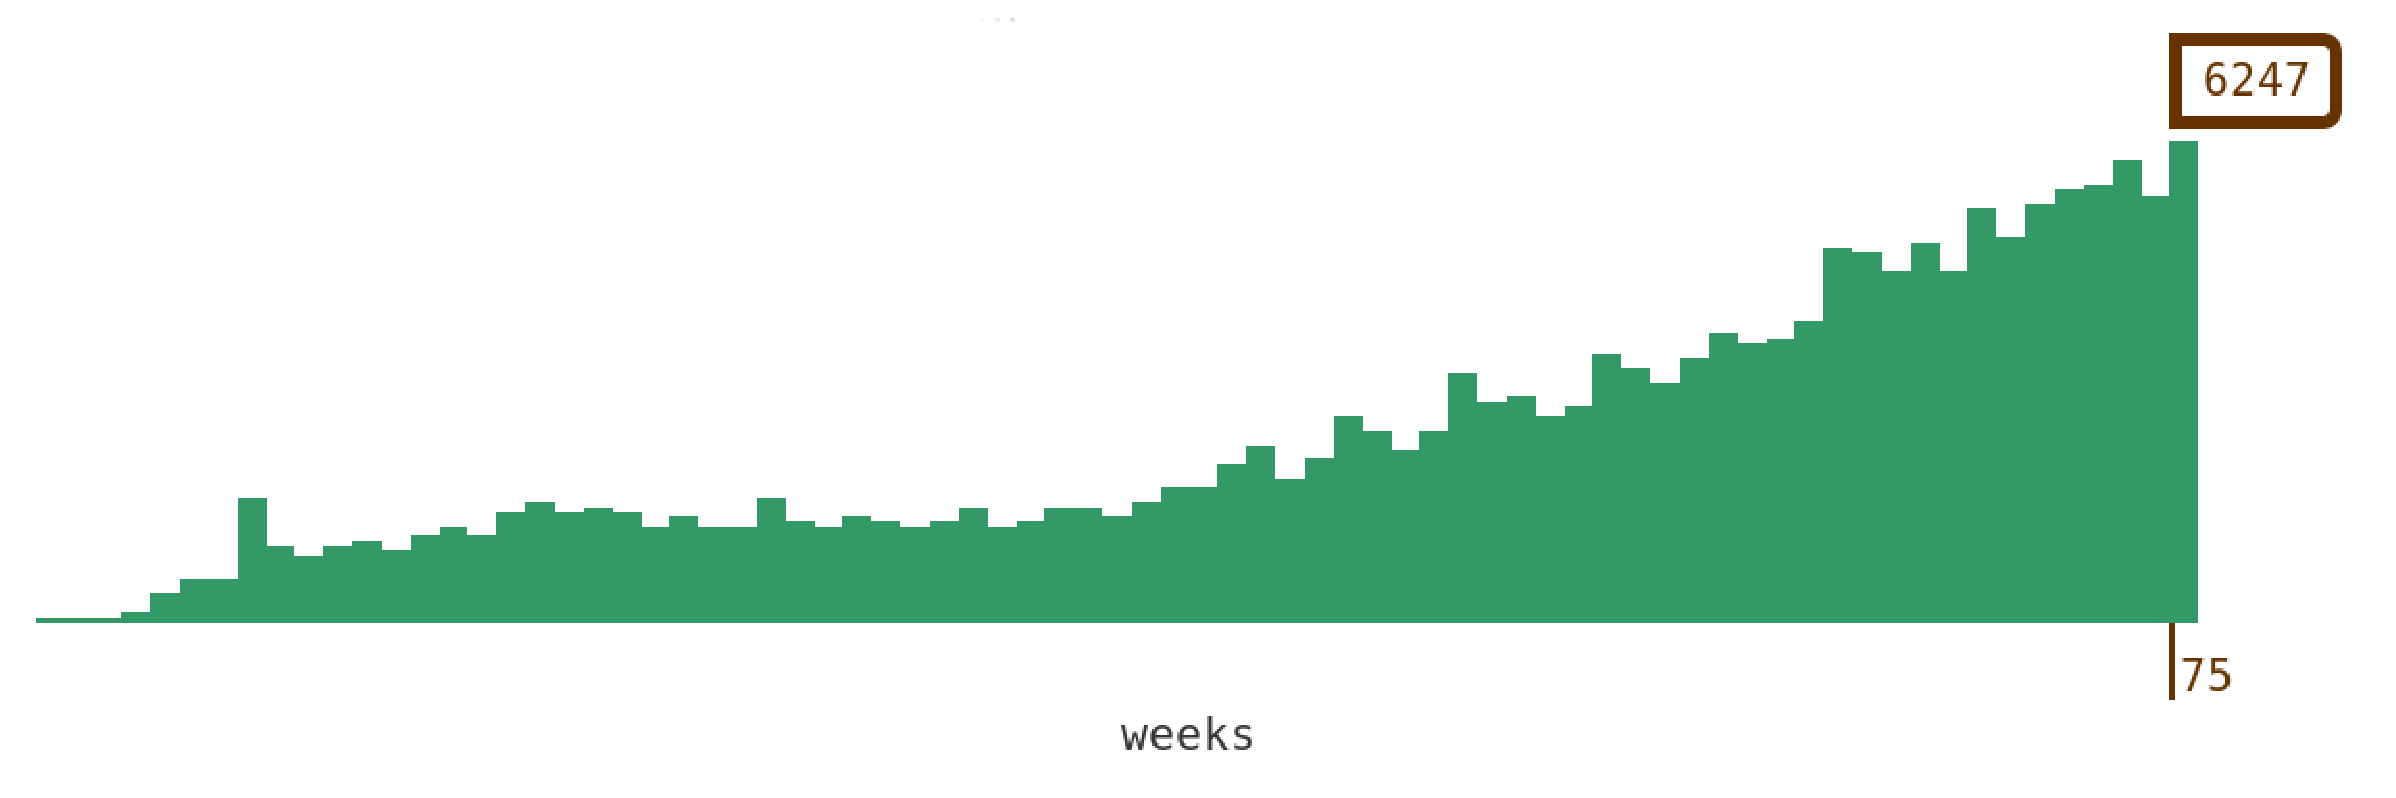
\includegraphics[width=16cm]{images/gittip-charges.eps}}
    \captionsource{Évolution des charges, en dollars, par semaine sur
        \url{gittip.com}}{\url{https://www.gittip.com/about/charts.html}}
\end{figure}

\paragraph{}
Début novembre 2013, si l'on compte 2 000 utilisateurs actifs sur
\url{gittip.com}, cela fait une moyenne de 3\${} de charges par utilisateur,
sur 3,5\${} échangés en moyenne. Ces charges restent importantes, et peut être
que Gittip devrait adopter un autre système de micropaiments en lignes qui
définisse des charges moins importantes à l'avenir. Pour le moment, Balance
Payments fait parti des systèmes open sources les moins couteux.

\subsection{la visibilité}

\paragraph{}
Lorsqu'un projet est inscrit sur une plateforme de financement communautaire,
il bénéficie de visibilité supplémentaire grace à son référencement. En effet,
les trois plateformes utilisées comme exemple, Kickstarter, Flattr et Gittip
disposent d'une liste de membres ou de projets classés par popularité.

\paragraph{}
La plateforme qui rend les projets les plus visibles est sans doute kickstarter
grâce à la sélection en page d'accueil des projets les plus proches
géographiquement ou les plus populaires du moment. Les projets sont classés par
catégories et par date de fin de manière a avantager les projets les plus
proches de l'échéance de financement. Les projets dont l'échéance est passée ne
sont plus mis en évidence.
Gittip peut être intéressant dans la mesure où la communauté reste assez
restreinte pour le moment; il est plus facile de se démarquer. Plus un projet
est financé, plus il occupe une position haute par catégorie.

\paragraph{}
L'utilisation conjuguée de kickstarter et gittip pourrait se révéler fructueuse
même en cas d'échec de la campagne kickstarter, pour faire connaître le projet.

\paragraph{}
Les modèle pay what you want fonctionne également, dans le cas du Humble Indie
Bundle pour mettre les jeux les moins connus en avant en les vendant dans la
même offre que des jeux plus populaires, le pic d'intérêt pour les internautes
étant créé par la popularité du site et le fait que les offres, plus
avantageuses que la normale, soient limité dans le temps.

%Ceci est encore une ébauche
\chapter{La problématique de la légalité du financement en France}\label{chapter3}
    \section{Introduction}
        \paragraph{}
            % Rappel des éléments précédents
            Nous avons jusqu'à présent étudié l'entrerpise et le site
            internet Gittip, ainsi que certains modèles de financements
            proposés pour pallier au problème du financement du logiciel
            libre, nous allons à présent nous intéresser plus en détail
            à l'aspect légal, et en particulier au volet fiscal, en relation
            avec l'utilisation des services proposés par gittip.
        \paragraph{}
            % Faire apparaître les 3 intervenants : le donneur, le receveur et gittip
            Avant tout, nous devrons distinguer les trois acteurs en jeu
            lors de l'utilisation du service de micro dons, et leurs rôles
            respectifs dans l'opération. 
            % Introduire le volet de fiscalité américaine
            Ensuite, gittip étant une société enregistrée aux États-unis
            il est nécessaire de se pencher brièvement sur son fonctionnement
            dans les conditions pour lesquelles son modèle a été pensé,
            c'est à dire le droit américain.
            % Droit français et conclusion
            Finalement, nous rentrerons dans le vif du sujet en détaillant les
            implications au niveau du droit fiscal français quant à
            l'utilisation des services proposés, et dresserons alors un bilan
            d'aptitude à l'utilisation de gittip en France

    \section{Généralités}
        \subsection{Acteurs}
            \paragraph{}
                Un don récurrent sur Gittip fait intervenir trois acteurs
                principaux.
                Tout d'abord le \emph{donateur}, de qui l'argent émane.
                Il s'agit le plus souvent d'un particulier, même si dans
                certains cas, il peut s'agir d'une organisation.
                Lorsque qu'il émet un don récurrent, gittip,
                l'\emph{intermédiaire} détermine si 
                le donateur possède suffisamment d'argent sur son compte,
                débite sa carte de crédit si nécessaire et procède au
                virement vers le compte gittip du \emph{donataire}. Ce dernier
                reçoit l'argent du donateur et peut ensuite le virer sur son
                compte bancaire ou l'utiliser pour faire lui-même un don.
                Nous utiliserons les concepts de donateur, intermédiaire et
                donataires tout au long de ce chapitre. 
    \section{Une entreprise américaine}
            % http://www.irs.gov/Businesses/Small-Businesses-%26-Self-Employed/Frequently-Asked-Questions-on-Gift-Taxes
            % http://www.irs.gov/pub/irs-prior/p950--2011.pdf
            % https://en.wikipedia.org/wiki/Commissioner_v._Duberstein
            %
            % Elements de droit américain. TL;DR : un donateur peut donner ce
            % qu'il veut à qui il veut tant que c'est sous 13.000$/an
            % 
            % Le donataire a rien à faire parce qu'à priori, c'est au donateur
            % au'incombent les taxes
            % 
            % Gittip doit envoyer un 1099K à l'IRS pour tout donateur au dessus de 20.000$/ans ET 200 transactions/ans
        \paragraph{}
            Les États-Unis sont une nation possédant une très forte cutlure
            du don. En effet, en favorisant l'autonomie vis à vis de leurs
            institutions gouvernantes, ce pays se base sur un grand nombre
            d'organisations de charités ayant pour but de donner aux citoyens
            les outils nécessaures à combattre les problèmes sociaux de leur
            société sans s'en remettre à un pouvoir politique, comme on
            pourrait le voir en France.
            D'autre part, le don est égallement un geste du quotidien :
            le tip (pourboire) pour rémunérer le service de divers
            professionnels tels que les chauffeurs de taxis, les serveurs ou
            encore les coiffeurs, n'est pas optionnel mais constitue une 
            obligation sociale.
            Dans ce contexte, la législation fiscale américaine est
            complète et permissive à ce sujet.
        \subsection{Donateur}
            Bien que l'IRS prévoit des taxes sur les dons, elles ne
            s'appliquent qu'à une fraction des cas de figures.
            Particulièrement, elles ne s'appliquent pas aux dons dont les
            donataires sont des parents du donateur, des organismes de
            charité ou des partis politiques, ni aux dons destinés à payer
            pour des dépenses médicales ou des frais d'éducation.
            De plus, pour les dons assujétis à la taxe sur les dons, il
            existe un large abattement annuel, fixé à 13000\dollar soit plus
            de 9500\euro pour l'année 2012. Si, malgré cela, les sommes
            données venaient à dépasser cet abattement, il reviendrait au
            donateur de s'acquitter de cette taxe.
        \subsection{Donataire}
            Comme nous l'avons vu, le poid fiscal repose, aux États-Unis, 
            sur les épaule du donateur. Cela est totalement transparent
            pour le donataire qui peut donc recevoir jusqu'à 13000\dollar
            par donateur par an sans que l'IRS ne s'intéresse à son cas.
        \subsection{Institution bancaire}
    \section{Utilisée par des français}
            % TL;DR beaucoup trop à dire là, voir mes notes
        \subsection{Donateur}
        \subsection{Donataire}
        \subsection{Institution bancaire}
    \section{Conclusion}

\chapter*{Conclusion}
\addcontentsline{toc}{chapter}{Conclusion}


% 1 Le modèle est intéressant et peut offrir une solution pour financer l'open source, de la façon Khan Academy
% 2 Le développement de la solution n'est pas encore optimal et comme toutes les grandes problématiques, il faudra du temps
% 3 La situation française rend l'accessibilité à ce modèle assez compliqué et il est à espérer que les choses changeront

Attendu les éléments que nous avons mis en avant, nous pouvons conclure notre
propos avec les points suivants.

\paragraph{}
Nous avons constaté le changement de point de vue qu'offre Gittip, du projet
dans les modèles de financement historiques vers l'individu.
Nous pensons que ce changement est pour le mieux et va dans la bonne
direction.
En effet, rémunérer les développeurs directement plutôt que de remplir les
caisses des projets sur lesquels ils travaillent permet d'offrir à ces
développeurs une motivation pour continuer à travailler comme ils le font, et
donc nous assure la pérennité de ces projets.
Il sera bien entendu nécessaire de faire en sorte que les finances propres des
projets permettent de payer pour leurs infrastructures, comme par exemple des
serveurs ou de la bande passante, mais là encore, Gittip permet cela par le
mécanisme des teams.

\paragraph{}
Nous exprimerons également notre enthousiasme sur la pratique de l'entreprise
Khan Academy de réserver un budget hebdomadaire par employé qui est donné par
le biais de Gittip à une personne du choix de l'employé en question.
Nous pensons qu'il s'agit d'une excellente façon pour une entreprise de
participer au financement du logiciel libre.

\paragraph{}
Ensuite, malgré cet enthousiasme, force est de constater que la solution
proposée laisse encore quelques points d'ombre. Par exemple, le montant gagné
par un développeur très visible mais peu efficace sera presque toujours plus
important que celui gagné par un développeur très efficace mais discret.
Il ne s'agit donc toujours pas du modèle parfait, et comme pour toute grande
problématique, la résolution de celle du financement du logiciel libre prendra
encore du temps.

\paragraph{}
Enfin, nous constatons que de notre côté de l'Atlantique, le système n'est pas
aussi viable qu'il pourrait l'être, à cause notamment de la faible culture du
don en France, du relatif vide juridique autour de la question, et des
difficultés fiscales rencontrées du fait de celui-ci. Il ne faut cependant pas
se montrer pessimiste : ce genre de barrières ont tendance à évoluer et si le
modèle de Gittip rencontre un grand succès dans d'autres pays, il n'est à
point douter que la France saura s'y adapter.

%% Pour tester l'exemple
%\chapter{Exemple}
    \section{Sous-exemple}

\lipsum[1-2]

    \subsection{Sous-sous-exemple}

\begin{itemize}
    \item Item exemple 1
    \item Item exemple 2
    \item Etc\ldots
\end{itemize}

\paragraph{}
J'écris des trucs dans un nouveau paragraphe.\\
Je vais même à la ligne.

Je peux aussi faire comme ça, et ça me fait un alinéa.

\paragraph{Liste à puces}
\begin{itemize}[label=\textbullet]
    \item Item exemple 1
    \item Item exemple 2
\end{itemize}

\paragraph{Tableau}
\begin{center}
\begin{tabular}{|c|c|c|}
    \hline % Permet d'avoir une séparation via un trait
    Colonne 1, ligne 1 & Colonne 2, ligne 1 & Colonne 3, ligne 1\\
    \hline
    Colonne 1, ligne 2 & Colonne 2, ligne 2 & Colonne 3, ligne 2\\
    Colonne 1, ligne 3 & Colonne 2, ligne 3 & Colonne 3, ligne 3\\
    \hline
    \multicolumn{2}{|c|}{Colonne 1 et 2, ligne 4} & Colonne 3, ligne 4\\
    \hline
\end{tabular}
\end{center}


%%% Table des matières

\tableofcontents
\addcontentsline{toc}{chapter}{Table des matières}

%%% Exemple pour les annexes
%\appendix
%\include{annexes/annexe1}
%\include{annexes/annexe2}

\end{document}
